\chapter{Approximate Spatial Searching}

\section{Introduction}

The {\bf approximate spatial searching} package implements
exact and approximate distance browsing
by providing implementations of algorithms supporting

\begin{itemize} 

\item
both nearest and furthest neighbour searching

\item
both exact and approximate searching

\item 
(approximate) $k$-nearest and $k$-furthest neighbour searching

\item 
(approximate) incremental nearest and incremental furthest neighbour searching

\item
query items representing points and spatial objects.

\end{itemize}

In these searching problems a set $P$ of data points in $d$-dimensional
space is given.
The points can be represented as Cartesian points or homogeneous points.
These points are preprocessed into a $k$-$d$ tree data structure, so that given
any query item $q$ the points of $P$ can be browsed efficiently.
The approximate spatial searching package is designed for data sets that are small enough to store
the search structure in main memory (in contrast to approaches
from databases that assume that the data reside in secondary storage).

\subsection{Spatial Searching}

Spatial searching supports browsing through a collection of spatial objects
stored in a spatial data structure on the basis of their distances to an arbitrary spatial
query object.
Spatial searching is supported in several ways. 
The first approach is $k$-{\bf nearest neighbour searching} that makes use of a $k$-nearest neighbour
algorithm, where $k$ is known prior to the invocation of the algorithm.
Hence, the number of nearest neighbours has to be
guessed. If the guess is too large redundant computations are performed.
If the number is too small the computation has to be  
reinvoked for a larger number of neighbours, thereby performing redundant computations.
The second approach is {\bf incremental nearest neighbour searching} in the sense that having obtained
the $k$ nearest neighbours, the $k$ + 1$^{st}$ neighbour can be obtained without
having to calculate the $k$ + 1 nearest neighbour from scratch.
The incremental approach is useful when processing queries where
one but not all of the conditions involves spatial proximity (e.g. the nearest city to Paris with
population greater than a million).

Spatial searching typically consists of a preprocssing phase and a searching phase. 
In the preprocessing phase one builds a search structure 
and in the searching phase 
one makes the queries. 
In the preprocessing phase the user builds a $k$-$d$ tree data structure storing the spatial data.
In the searching phase the user invokes a searching method to browse the spatial data.

With relatively minor modifications, nearest neighbour searching algorithms can be
used to find the furthest object from the query object. 
Therefore, {\bf Furthest neighbour searching} is also supported
by the approximate spatial searching package.

{\bf Range searching}
is supported for $d$-dimensional rectangles and spheres using incremental nearest neighbour search. 
Rectangular range queries are supported by 
using iso-rectangles as query item, and using a $L1$-distance between iso-rectangles and points.
Spherical range queries are supported by using spheres as query item, and using a $L2$-distance
between spheres and points.
In both cases the distance is defined such that all points contained in a query item have distance zero
to the query item. Hence, an incremental nearest neighbour search will report first all points
contained in the query item.  

{\bf Approximate searching}, is supported by
specifying an approximation factor $\epsilon \geq 0$ with the query.

\subsection{The $k$-$d$ tree}
\label{KDT_section}

Bentley \cite{b-mbstu-75} introduced the $k$-$d$ tree as a generalization of the binary
search tree in higher dimensions. $k$-$d$ trees hierarchically decompose space into a
relatively small number of rectangles such that no rectangle contains too many input objects.
For our purposes, a {\it rectangle} in real $d$ dimensional space, $\R^d$, is the product of $d$ closed
intervals on the coordinate axes.
$k$-$d$ trees are obtained by partitioning point sets in $\R^d$ using
($d$-1)-dimensional hyperplanes.
Each node in the tree is split into two children by one such separating hyperplane.

Each internal node of the $k$-$d$ tree is associated with a rectangle
and a hyperplane orthogonal to
one of the coordinate axis, which splits the rectangle into two parts.
Therefore, such a hyperplane, defined by a splitting dimension
and a splitting value, is called a separator.
These two parts are then associated
with the two child nodes in the tree. The process of partitioning space continues until the number of data
points in the rectangle falls below some given threshold. The rectangles associated with the leaf nodes
are called {\it buckets}, and they define a subdivision of the space into rectangles.
Data points are only stored in the leaf nodes of the tree, not in the internal nodes.

Friedmann, Bentley and Finkel \cite{fbf-afbml-77} described the standard
search algorithm to find the $k$th nearest neighbour by searching a $k$-$d$ tree recursively.

When encountering a node of the  the algorithm first visits the child that is closest
to the query point. On return, if the rectangle containing  the other child lies within
1/ (1+$\epsilon$) times the distance to the $k$th nearest neighbours so far, then
the other child is visited recursively.
Priority search \cite{am-annqf-93} visits the nodes in increasing order of distance from
the queue with help of a priority queue.
The search stops when the distance of the query point to the nearest nodes
exceeds the distance to the nearest point found with a factor 1/ (1+$\epsilon$).
Priority search supports next neighbour search, standard search does not.

In order to speed-up the internal distance computations in nearest neighbour searching
in high dimensional space, the approximate searching package supports orthogonal searching. Orthogonal
searching implements the efficient incremental distance computation
technique introduced by Arya and Mount \cite{am-afvq-93}.
Orthogonal searching works only for nearest neighbour queries using query items representing
points. Also the use of a Minkowski distance is required.

To speed up distance computations also transformed
distances are used instead of the distance itself. 
For instance for the Euclidean distance, to avoid the expensive computation
of square roots, squared distances are used instead of the Euclidean distance itself. 

\section{Example Programs}

We give five examples. 
The first example illustrates nearest neighbour searching.
Approximate searching is illustrated by the second example and range
searching is illustrated by the third example.
The fourth example illustrates distance browsing and the last example illustrates using
a user defined point and distance class.

\subsection{Example of Nearest Neighbour Searching}

The first example illustrates nearest neighbour searching. The random data points are preprocessed
in a $k$-$d$ tree. For each of the random query points its nearest neighbour is obtained.
For the Euclidean distance used in this example \ccc{inverse_of_transformed_distance}
implements taking the square root. (See also the last remark at the end of section~\ref{KDT_section}.)


\ccIncludeExampleCode{ExampleA.C}

\subsection{Example of Approximate Nearest and Furthest Neighbour Searching}

The second example program illustrates approximate nearest neighbour searching
using 4-dimensional Cartesian coordinates.
In this example the \ccc{MEDIAN_OF_MAX_SPREAD} splitting rule instead of the default splitting
rule is used to build the $k$-$d$ tree. Five approximate nearest and furthest neighbours of
the query point (0.0, 0.0, 0.0, 0.0) are computed.
 
\ccIncludeExampleCode{ExampleB.C}

\subsection{Example of a Range Query}

The third example program illustrates range querying using homogeneous 3-dimensional coordinates. 
A range query is defined by an instance of \ccc {CGAL::Iso_cuboid_3}. 
All items in a range query are retrieved by 
\ccc{get_elements_in_query}, which computes all items in
the range query by appling incremental nearest neighbour searching. 

\ccIncludeExampleCode{ExampleC.C}

The fourth example program illustrates browsing for $4$-dimensional points with
a positive first coordinate using orthogonal priority search
using the point class \ccc{CGAL::Point_d}
and the distance class \ccc{CGAL::Weighted_Minkowski_distance}.
 
\subsection{Example of distance browsing}

\ccIncludeExampleCode{ExampleD.C}

This example illustrates distance browsing to find the first 10 nearest neighbours of which
the first coordinate is positive. 

\subsection{Example illustrating use of user defined point and distance class}

In this example the user provides an implementation of 3-dimensional points and an
implementation of the Euclidean distance.

\ccIncludeExampleCode{ExampleE.C}

\section{Classes}

A user of the approximate spatial searching package should consult the reference
pages of the following classes

\begin{itemize}

\item
The class \ccc{Kd_tree} implementing the $k$-$d$ tree.

\item
The class \ccc{Kd_tree_traits_point} providing parameters for the construction of the $k$-$d$ tree.

\item
The class \ccc{Weighted_Minkowski_distance} implementing a weighted $L_p$-distance for $d$-dimensional points.

\item
The class \ccc{L1_distance_rectangle_point} implementing a $L1$ distance for $d$-dimensional
iso-rectangles and points. 

\item
The class \ccc{L2_distance_sphere_point} implementing a $L2$ distance for $d$-dimensional
spheres and points. 

\item
The class \ccc{General_standard_search} implementing the standard search strategy for general distances
like the $L1$ distance for iso-rectangles.

\item
The class \ccc{General_priority_search} implementing the priority search strategy for general distances
like the $L1$ distance for iso-rectangles.

\item
The class \ccc{Orthogonal_standard_search} implementing the standard search strategy for orthogonal distances
like a weighted $L_p$ distance. Requires the use of extended nodes in the $k$-$d$ tree and supports
only approximate nearest neighbour searching for point queries.

\item
The class \ccc{Orthogonal_priority_search} implementing the priority search strategy for general distances
like the $L1$ distance for iso-rectangles. Requires the use of extended nodes in the $k$-$d$ tree
and supports
only approximate nearest neighbour searching for point queries.

\item
If a user wants to define a distance class the part of the reference page of the class
\ccc{Kd_tree_rectangle} that is not marked as advanced section.
 
\end{itemize}

\section{Use of traits classes}

\begin{figure}[t]
\begin{ccTexOnly}
\begin{center}
\leavevmode
\vspace*{6cm}
\hspace*{-2cm}
\scalebox{.7}{\includegraphics{Fig1.eps}}
\end{center}
\vspace*{-8cm}
\end{ccTexOnly}
\caption{Overview of use of traits classes.
\label{ASPAS:Fig1}}
\end{figure}

\begin{ccHtmlOnly}
% <CENTER>
% <img border=0 src=Fig1.gif align=center alt="Overview of use of traits classes">
% </CENTER>
% after kdtree
<P>
<center>
<img border=0 src="./Fig1.gif" alt=" "><br> 
Overview of use of traits classes.</center>
\end{ccHtmlOnly}




Figure \ref{ASPAS:Fig1} shows an overview of the use of the traits classes.

The parameter \ccc{NT} should provide a number type.

The parameter \ccc{Item} should provide an implementation of a $d$-dimensional point, 
for example \ccc{CGAL::Point_d}.

The parameter \ccc{Query_item} should provide an implementation a spatial object
as specified by the concept \ccc{CGAL::QueryItem}
for example \ccc{CGAL::Kd_tree_rectangle}, that implements $d$-dimensional iso rectangles.

The parameter \ccc{Separator} should provide an implementation of a $d-1$-dimensional
subspace as specified by the concept \ccc{CGAL::Separator}.

The parameter \ccc{Traits} should provide an implementation of the concept \ccc{CGAL::TreeTraits}
specifying the parameters and the splitting rule used in the construction of a $k$-$d$ tree.

The parameter \ccc{Distance} should provide an implementation of a distance.
For the implementation of nearest neighbour searching with efficient incremental
distance computation this distance class should meet the requirements of the concept
\ccc{CGAL::OrthogonalDistance}. Otherwise the distance class has only to meet the
requirements of the concept \ccc{CGAL::GeneralDistance}.


\section{Splitting Rules}

Instead of using the default splitting rule \ccc{Sliding_midpoint} described below,
an advanced user may, depending upon the data, select 
using an instance from the enumeration \ccc{Split_rules}
one from the following splitting rules,
which determine how a separating hyperplane is selected:

\begin{itemize}

\item \ccc{Midpoint_of_rectangle}

This splitting rule cuts a rectangle through its midpoint orthogonal
to the longest side.

\item \ccc{Midpoint_of_max_spread}

This splitting rule cuts a rectangle through $(Mind+Maxd)/2$ orthogonal
to the dimension with the maximum point spread $[Mind,Maxd]$.

\item \ccc{Sliding_midpoint}

This is a modification of the midpoint of rectangle splitting rule.
It first attempts to perform a midpoint of rectangle split as
described above. If data points lie on both sides of the separating
plane the sliding midpoint rule computes the same separator as
the midpoint of rectangle rule. If the data points lie only on one
side it avoids this by sliding the separator, computed by
the midpoint of rectangle rule, to the nearest datapoint.

\item \ccc{Median_of_rectangle}

The splitting dimension is the dimension of the longest side of the rectangle.
The splitting value is defined by the median of the coordinates of the data points
along this dimension.

\item \ccc{Median_of_max_spread}

The splitting dimension is the dimension of the longest side of the rectangle.
The splitting value is defined by the median of the coordinates of the data points
along this dimension.

\item \ccc{Fair}

This splitting rule is a compromise between the median of rectangle splitting rule
and the midpoint of rectangle splitting rule. This splitting rule maintains an upper
bound on the maximal allowed ratio of the longest and shortest side of
a rectangle (the value of this upper bound is set in the constructor of the
fair splitting rule). Among the splits that satisfy this bound, it selects
the one in which the points have the largest spread.
It then splits the points in the most even manner possible, subject
to maintaining the bound on the ratio of the resulting rectangles.

\item \ccc{Sliding_fair}

This splitting rule is a compromise between the fair splitting rule
and the sliding midpoint rule.
Sliding fair-split is based on the theory that there are
two types of splits that are good: balanced splits that
produce fat rectangles, and unbalanced splits provided
the rectangle with fewer points is fat.

Also, this splitting rule maintains an upper
bound on the maximal allowed ratio of the longest and shortest side of
a rectangle (the value of this upper bound is set in the constructor of the
fair splitting rule). Among the splits that satisfy this bound, it selects
the one one in which the points have the largest spread.
It then considers the most extreme cuts that would be allowed by the
aspect ratio bound. This is done by dividing the longest side of
the rectangle by the aspect ratio bound. If the median cut lies
between these extreme cuts, then we use the median cut. If not,
then consider the extreme cut that is closer to the median.
If all the points lie to one side of this cut, then we slide the cut
until it hits the first point.
This may violate the aspect ratio bound, but will never generate empty cells.

\end{itemize}

Also, a user may provide an implementation of his own
splitting rule.

\section{Implementation}

The following classes are only of interest for modifying the implementation of the
approximate spatial searching package. Their reference pages are described as advanced sections.

\begin{itemize}

\item
The class \ccc{Kd_tree_rectangle} implements $d$-dimensional iso-rectangles, 
methods to compute bounding boxes
of point sets and methods to split iso-rectangles.

\item
The class \ccc{Kd_tree_node} implements $k$-$d$ tree nodes.

\item
The class \ccc{Plane_separator} implements a separator.

\item 
The class \ccc{Point_container} is a point container providing a method, that given a separator
splits a point set. Also \ccc{Point_container} provides methods that support the implementation
of splitting rules.

\item
The function object classes \ccc{Midpoint_of_rectangle}, \ccc{Midpoint_of_max_spread},
\ccc{Sliding_midpoint}, \ccc{Median_of_rectangle}, \ccc{Median_of_max_spread}, \ccc{Median_of_max_spread},
\ccc{Fair} and \ccc{Sliding_fair} implement the splitting rules.

\end{itemize}
